% Copyright (c) Patrick Hall (jphall@gwu.edu), 2026-27. CC BY-NC-SA 4.0.
\documentclass[aspectratio=169]{beamer}
\usetheme{Singapore}
\definecolor{brand}{RGB}{45,110,191}
\definecolor{hrgray}{RGB}{100,100,100}
\definecolor{sourcegray}{RGB}{90,90,90}
\setbeamercolor{structure}{fg=brand}
\setbeamercolor{title}{fg=hrgray}
\setbeamercolor{subtitle}{fg=brand}
\setbeamercolor{frametitle}{fg=hrgray}
\setbeamercolor{block title}{fg=white,bg=brand}
\setbeamercolor{block body}{bg=black!2}
\usepackage[T1]{fontenc}
\usepackage[utf8]{inputenc}
\usepackage{lmodern,microtype,graphicx,booktabs,tabularx,array,tikz,amsmath}
\usepackage[backend=biber,style=authoryear,maxcitenames=2,maxbibnames=10,doi=false,isbn=false,url=true]{biblatex}
\addbibresource{references.bib}
\renewcommand*{\bibfont}{\scriptsize}
\usetikzlibrary{positioning,arrows.meta,shapes.geometric,fit,calc}
\setbeamertemplate{navigation symbols}{}
\setbeamertemplate{bibliography item}{}
\setbeamertemplate{frametitle continuation}{}
\setbeamertemplate{footline}{\leavevmode\hbox{\begin{beamercolorbox}[wd=.5\paperwidth,ht=3ex,dp=1ex,left]{author in head/foot}\hspace{0.8ex}
\includegraphics[height=.5cm]{../../asset/gw_logo.png}\end{beamercolorbox}\begin{beamercolorbox}[wd=.5\paperwidth,ht=3ex,dp=1ex,right]{date in head/foot}\insertframenumber/\inserttotalframenumber\hspace{2ex}\end{beamercolorbox}}}
\title{Lecture 5: RAG and knowledge pipelines}
\subtitle{From source documents to grounded, cited answers}
\author[Patrick Hall]{\textbf{Patrick Hall}}
\institute{Department of Decision Sciences}
\date{\today}
\newcommand{\slidesource}[1]{\par\vfill\noindent\parbox{\linewidth}{\tiny\color{sourcegray}\raggedright\sloppy Source: #1.}}
\newcommand{\visualdescription}[1]{\par\vspace{.2em}\noindent\parbox{\linewidth}{\centering\tiny\color{sourcegray}#1}}
\newcommand{\R}{\mathbb{R}}
\newcolumntype{Y}{>{\raggedright\arraybackslash}X}

\begin{document}

\begin{frame}
  \titlepage
  \vspace{-.75em}
  \centering\scriptsize \textcopyright\ 2026--27 Patrick Hall (jphall@gwu.edu). Some rights reserved. Text and copy are licensed under a \href{https://creativecommons.org/licenses/by-nc-sa/4.0/}{Creative Commons Attribution-NonCommercial-ShareAlike 4.0 International License (CC BY-NC-SA 4.0)}.
  \begin{tikzpicture}[remember picture,overlay]
    \node[opacity=.08] at (current page.center) {
\includegraphics[width=.55\paperwidth]{../../asset/gw_logo.png}};
  \end{tikzpicture}
\end{frame}

\begin{frame}{Agenda}
  \tableofcontents
\end{frame}

\section{What RAG changes}
\begin{frame}{RAG adds an explicit, inspectable knowledge path}
\small
\begin{columns}[c]
\column{.49\textwidth}
\begin{block}{Retrieval-augmented generation}
At answer time, retrieve relevant passages from a specialized document corpus, add them to the model context, and generate an answer constrained by those passages \parencite{Lewis2020RAG}.
\end{block}
\begin{itemize}\itemsep0pt\parsep0pt\topsep0pt
\item \textbf{Specialize answers} around trusted documents such as policies, manuals, research, or product records.
\item \textbf{Reduce hallucination risk} by grounding answers in retrieved evidence; relevance and citation support must still be checked.
\item \textbf{Enable citation} through passage-level source IDs and links.
\end{itemize}
\column{.47\textwidth}
\centering
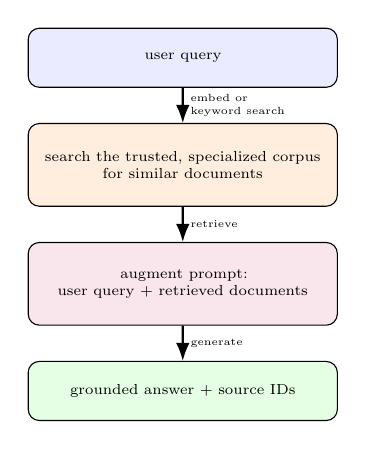
\begin{tikzpicture}[scale=.75,transform shape,node distance=6mm,>=Latex,every node/.style={font=\scriptsize,align=center}]
\node[draw,rounded corners,fill=blue!8,text width=50mm,minimum height=10mm] (q) {user query};
\node[draw,rounded corners,fill=orange!13,text width=50mm,minimum height=14mm,below=of q] (search) {search the trusted, specialized corpus\\for similar documents};
\node[draw,rounded corners,fill=purple!10,text width=50mm,minimum height=14mm,below=of search] (prompt) {augment prompt:\\user query + retrieved documents};
\node[draw,rounded corners,fill=green!10,text width=50mm,minimum height=10mm,below=of prompt] (answer) {grounded answer + source IDs};
\draw[->,thick] (q)--node[right,font=\tiny,align=left]{embed or\\keyword search} (search);
\draw[->,thick] (search)--node[right,font=\tiny]{retrieve} (prompt);
\draw[->,thick] (prompt)--node[right,font=\tiny]{generate} (answer);
\end{tikzpicture}
\visualdescription{A query and retrieved documents form an augmented prompt that produces a grounded answer with source IDs.}
\end{columns}
\end{frame}

\section{Build the knowledge pipeline}
\begin{frame}{Ingestion makes a source usable and accountable}
\small
\begin{columns}[c]
\column{.54\textwidth}
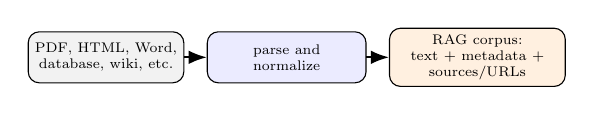
\begin{tikzpicture}[scale=.72,transform shape,>=Latex,node distance=4mm,every node/.style={font=\scriptsize,align=center}]
\node[draw,rounded corners,fill=gray!10,minimum width=25mm,minimum height=9mm] (raw) {PDF, HTML, Word,\\database, wiki, etc.};
\node[draw,rounded corners,fill=blue!8,minimum width=28mm,minimum height=9mm,right=of raw] (parse) {parse and\\normalize};
\node[draw,rounded corners,fill=orange!12,minimum width=31mm,minimum height=9mm,right=of parse] (record) {RAG corpus:\\text + metadata +\\sources/URLs};
\draw[->,thick] (raw)--(parse); \draw[->,thick] (parse)--(record);
\end{tikzpicture}
\visualdescription{Source files are parsed into a RAG corpus that preserves text, metadata, and links to the originating source.}
\par\vspace{.8em}\footnotesize\raggedright Keep a stable source ID, version or retrieval date, access-control label, title, section, and canonical URL. These fields make later citations and audits possible.
\column{.42\textwidth}
\begin{block}{Ingestion checks}
\begin{itemize}\itemsep.25em
\item Is the source authorized and current?
\item Did extraction retain headings, tables, and links?
\item Can each chunk lead a reader back to the original source?
\end{itemize}
\end{block}
\end{columns}
\end{frame}

\begin{frame}{Fixed-length chunking trades context, recall, and attribution}
\small
\begin{columns}[T]
\column{.56\textwidth}
{\scriptsize\raggedright
\textbf{Fixed-length chunks from AI RMF GOVERN 1.1--1.6 \parencite{NIST2023AIRMF}}\\[.2em]
\fcolorbox{brand}{blue!5}{\parbox{.93\linewidth}{\tiny
\textbf{Chunk 1 \textbar{} begins at GOVERN 1.1; 128-token cutoff}\\
\textbf{GOVERN 1.1} Legal and regulatory requirements involving AI are understood, managed, and documented. \textbf{GOVERN 1.2} The characteristics of trustworthy AI are integrated into organizational policies, processes, procedures, and practices. \textbf{GOVERN 1.3} Processes, procedures, and practices are in place to determine the needed level of risk management activities based on the organization's risk tolerance. \textbf{GOVERN 1.4} The risk management process and its outcomes are established through transparent policies, procedures, and other controls based on organizational risk priorities. \textbf{GOVERN 1.5} Ongoing monitoring and periodic review of the risk management process and its outcomes are planned and organizational roles and responsibilities\ \textcolor{red!70!black}{\textbf{[cutoff]}}}}\\[.45em]
\fcolorbox{brand}{green!10}{\parbox{.93\linewidth}{\tiny
\textbf{Chunk 2 \textbar{} 16 repeated tokens + new tokens}\\
\textcolor{orange!80!black}{\textbf{[repeat 16]}} \emph{review of the risk management process and its outcomes are planned and organizational roles and responsibilities}. \textcolor{green!50!black}{\textbf{[new]}} \textbf{GOVERN 1.5} clearly defined, including determining the frequency of periodic review. \textbf{GOVERN 1.6} Mechanisms are in place to inventory AI systems and are resourced according to organizational risk priorities\ldots}}
\par\vspace{.05em}\parbox{.93\linewidth}{\tiny\raggedright The boundary is tokenizer-specific; here it visibly divides GOVERN 1.5 rather than respecting its subcategory boundary.}
}
\column{.40\textwidth}
\scriptsize
\begin{block}{Sizing and overlap heuristic}
\begin{itemize}\itemsep.2em
\item Start from a meaningful record; do not split a record that is already shorter than the target size.
\item Use shorter chunks (for example, 128 tokens) for detail and citation locality; use larger chunks for themes and summaries.
\item Use 10--20\% overlap for ordinary prose. Here, $16/128=12.5\%$; raise it for boundary-crossing clauses, tables, or lists.
\item Test size, overlap, retrieval depth $k$, and answer faithfulness \parencite{Lewis2020RAG}.
\end{itemize}
\end{block}
\end{columns}
\end{frame}

\begin{frame}{Semantic chunking respects structure and meaning}
\small
\begin{columns}[c]
\column{.54\textwidth}
{\tiny\raggedright
\textbf{AI RMF GOVERN records as structure-aligned chunks \parencite{NIST2023AIRMF}}\\[.2em]
\fcolorbox{brand}{blue!5}{\parbox{.93\linewidth}{\textbf{Chunk 1 \textbar{} GOVERN 1.1} Legal and regulatory requirements involving AI are understood, managed, and documented.}}\\[.25em]
\fcolorbox{brand}{orange!10}{\parbox{.93\linewidth}{\textbf{Chunk 2 \textbar{} GOVERN 1.2} The characteristics of trustworthy AI are integrated into organizational policies, processes, procedures, and practices.}}\\[.25em]
\fcolorbox{brand}{green!10}{\parbox{.93\linewidth}{\textbf{Chunk 3 \textbar{} GOVERN 1.3} Processes, procedures, and practices are in place to determine the needed level of risk management activities based on the organization's risk tolerance.}}\\[.25em]
\fcolorbox{brand}{purple!10}{\parbox{.93\linewidth}{\textbf{Chunk 4 \textbar{} GOVERN 1.4} The risk management process and its outcomes are established through transparent policies, procedures, and other controls based on organizational risk priorities.}}\\[.25em]
\fcolorbox{brand}{blue!5}{\parbox{.93\linewidth}{\textbf{Chunk 5 \textbar{} GOVERN 1.5} Ongoing monitoring and periodic review of the risk management process and its outcomes are planned and organizational roles and responsibilities clearly defined, including determining the frequency of periodic review.}}\\[.25em]
\fcolorbox{brand}{orange!10}{\parbox{.93\linewidth}{\textbf{Chunk 6 \textbar{} GOVERN 1.6} Mechanisms are in place to inventory AI systems and are resourced according to organizational risk priorities.}}\\[.35em]
\centering\ldots
}
\column{.42\textwidth}
\footnotesize
\begin{itemize}\itemsep.45em
\item Use clear document structure when available: headings, sections, table rows, enumerated controls, or other authored boundaries.
\item When structure is weak, embed adjacent sentences or paragraphs and start a new chunk when similarity falls below a calibrated threshold \parencite{Karpukhin2020DPR}.
\item Retain the heading and source ID, and enforce practical minimum and maximum chunk lengths.
\item An embedding boundary is not automatically a meaningful policy, legal, or table boundary. Inspect failures.
\end{itemize}
\end{columns}
\end{frame}

\section{Retrieve and rank}
\begin{frame}{Embeddings represent query--passage similarity}
\small
\begin{columns}[c]
\column{.53\textwidth}
For a query $q$ and chunks $d_j$, an embedding model maps text to vectors:
\[
\begin{aligned}
e(q),e(d_j)&\in\R^D,\\[-.15em]
s_{\mathrm{dense}}(q,d_j)&=\frac{e(q)^\top e(d_j)}{\lVert e(q)\rVert_2\lVert e(d_j)\rVert_2}.
\end{aligned}
\]
Rank chunks by $s_{\mathrm{dense}}$ and preserve each chunk's source metadata. Dense retrieval can match related language even when query and passage do not share exact terms \parencite{Karpukhin2020DPR,OpenAI2026Embeddings}.
\column{.43\textwidth}
\centering
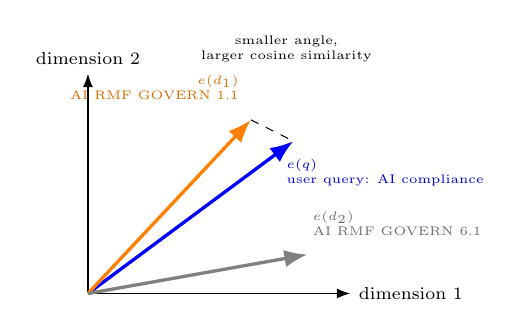
\begin{tikzpicture}[scale=.90,transform shape,>=Latex,every node/.style={font=\scriptsize,align=center}]
\draw[->] (0,0)--(3.7,0) node[right] {dimension 1};
\draw[->] (0,0)--(0,3.1) node[above] {dimension 2};
\draw[->,very thick,blue] (0,0)--(2.9,2.15);
\draw[->,very thick,orange] (0,0)--(2.3,2.45);
\draw[->,very thick,gray] (0,0)--(3.1,.55);
\draw[dashed] (2.3,2.45)--(2.9,2.15);
\node[text=orange!85!black,font=\tiny,align=right,anchor=south east] at (2.25,2.62) {$e(d_1)$\\AI RMF GOVERN 1.1};
\node[text=blue!80!black,font=\tiny,align=left,anchor=north west] at (2.68,2.02) {$e(q)$\\user query: AI compliance};
\node[text=gray!85!black,font=\tiny,align=left,anchor=south west] at (3.05,.70) {$e(d_2)$\\AI RMF GOVERN 6.1};
\node[font=\tiny,align=center] at (2.8,3.45) {smaller angle,\\larger cosine similarity};
\end{tikzpicture}
\visualdescription{An AI-compliance query embedding lies closer in direction to the GOVERN 1.1 embedding than to the GOVERN 6.1 embedding; cosine similarity compares those directions.}
\end{columns}
\end{frame}

\begin{frame}{Hybrid search combines complementary signals}
\small
\begin{columns}[c]
\column{.54\textwidth}
\centering
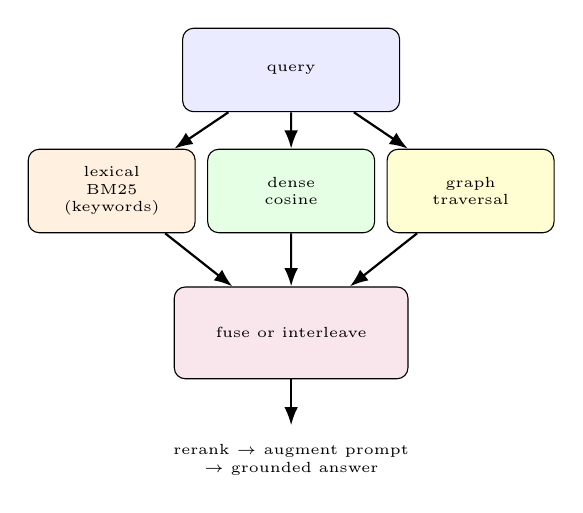
\begin{tikzpicture}[scale=1.06,transform shape,>=Latex,every node/.style={font=\tiny,align=center}]
\node[draw,rounded corners,fill=blue!8,minimum width=26mm,minimum height=10mm] (q) at (0,0) {query};
\node[draw,rounded corners,fill=orange!12,minimum width=20mm,minimum height=10mm] (lex) at (-2.15,-1.45) {lexical\\BM25\\(keywords)};
\node[draw,rounded corners,fill=green!10,minimum width=20mm,minimum height=10mm] (dense) at (0,-1.45) {dense\\cosine};
\node[draw,rounded corners,fill=yellow!18,minimum width=20mm,minimum height=10mm] (graph) at (2.15,-1.45) {graph\\traversal};
\node[draw,rounded corners,fill=purple!10,minimum width=28mm,minimum height=11mm] (fuse) at (0,-3.15) {fuse or interleave};
\draw[->,thick] (q)--(lex); \draw[->,thick] (q)--(dense); \draw[->,thick] (q)--(graph); \draw[->,thick] (lex)--(fuse); \draw[->,thick] (dense)--(fuse); \draw[->,thick] (graph)--(fuse);
\draw[->,thick] (fuse.south) -- ++(0,-.55) node[below=1mm,font=\tiny,align=center] {rerank $\rightarrow$ augment prompt\\$\rightarrow$ grounded answer};
\end{tikzpicture}
\visualdescription{Lexical, dense, and graph retrieval candidates are fused.}
\column{.42\textwidth}
\begin{itemize}\itemsep.3em
\item Lexical search is strong for exact control IDs, names, and rare terms.
\item Dense search is strong for paraphrases and related meanings.
\item GraphRAG can surface connected entities, relationships, or community-level context when an answer spans passages \parencite{Edge2024GraphRAG,MicrosoftGraphRAG2026}.
\item Normalize or combine ranks before comparing scores from different systems \parencite{Robertson2009BM25,Karpukhin2020DPR}.
\end{itemize}
\end{columns}
\end{frame}

\begin{frame}{Reranking spends more computation on fewer candidates}
\small
\begin{columns}[c]
\column{.54\textwidth}
\centering
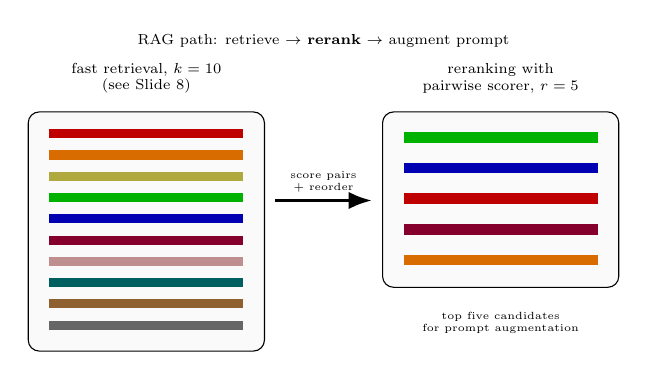
\begin{tikzpicture}[scale=.75,transform shape,>=Latex]
\node[font=\scriptsize,align=center] at (5,5.25) {RAG path: retrieve $\rightarrow$ \textbf{rerank} $\rightarrow$ augment prompt};
\node[font=\scriptsize,align=center] at (2,4.62) {fast retrieval, $k=10$\\(see Slide 8)};
\node[font=\scriptsize,align=center] at (8,4.62) {reranking with\\pairwise scorer, $r=5$};
\draw[rounded corners,fill=gray!4] (0,0) rectangle (4,4.05);
\draw[rounded corners,fill=gray!4] (6,1.08) rectangle (10,4.05);
\foreach \y/\c in {3.68/red!75!black,3.32/orange!85!black,2.96/yellow!65!black,2.60/green!70!black,2.24/blue!70!black,1.88/purple!70!black,1.52/pink!75!black,1.16/teal!75!black,.80/brown!75!black,.44/gray!80!black}
  {\draw[\c,line width=1.15mm] (.36,\y)--(3.64,\y);}
\foreach \y/\c in {3.62/green!70!black,3.10/blue!70!black,2.58/red!75!black,2.06/purple!70!black,1.54/orange!85!black}
  {\draw[\c,line width=1.35mm] (6.36,\y)--(9.64,\y);}
\draw[->,very thick] (4.18,2.55)--node[above,font=\tiny,align=center]{score pairs\\+ reorder} (5.82,2.55);
\node[font=\tiny,align=center] at (8,.48) {top five candidates\\for prompt augmentation};
\end{tikzpicture}
\visualdescription{Ten fast-retrieval candidates are scored against the query and reordered; the five highest-ranked candidates continue to prompt augmentation.}
\column{.42\textwidth}
\begin{itemize}\itemsep.35em
\item A cross-encoder is a Transformer encoder (such as BERT) that reads the query and one candidate document together, then outputs a relevance score; an LLM judge can play a similar role.
\item Reranking is more expensive than first-stage retrieval, so apply it only to a small candidate set.
\item Compare recall@$k$, ranking quality, latency, and support for final claims on held-out questions \parencite{Nogueira2019Reranking}.
\end{itemize}
\end{columns}
\end{frame}

\section{Generate, cite, and operate}
\begin{frame}{Grounded generation makes use of clear contracts}
\small
\begin{columns}[t]
\column{.52\textwidth}
\begin{block}{System prompt instruction}
\scriptsize
\texttt{\# Grounded-answer policy}\par\vspace{-.15em}
\texttt{- Use only the **Retrieved context** below.}\\
\texttt{- Add [source ID] after every factual claim.}\\
\texttt{- If unsupported, say: "I don't have enough evidence."}
\end{block}
\begin{block}{Example retrieved context}
\scriptsize
\texttt{[MS-2.1] Test sets, metrics, and details about the tools used during testing, evaluation, verification, and validation are documented.}\\[.35em]
\texttt{[MG-4.1] Post-deployment AI-system monitoring plans include mechanisms for user and stakeholder input, appeal and override, decommissioning, incident response, recovery, and change management.}
\end{block}
\column{.44\textwidth}
\begin{block}{Example cited answer}
\footnotesize
\textit{Question: What should an organization document and include in its monitoring plan?}\\[.35em]
Document the test sets, metrics, and tools used during testing, evaluation, verification, and validation (TEVV) \texttt{[MS-2.1]}. Include user input, appeals, incident response, recovery, and change management in the monitoring plan \texttt{[MG-4.1]}.
\par\vspace{.45em}
\scriptsize\textbf{References:} \\
\texttt{[MS-2.1]} NIST AI RMF Playbook, Measure 2.1.\\
\texttt{[MG-4.1]} NIST AI RMF Playbook, Manage 4.1.
\end{block}
\end{columns}
\end{frame}

\begin{frame}{Citations need coverage and correctness checks}
\small
\begin{columns}[c]
\column{.52\textwidth}
\begin{tabularx}{\linewidth}{>{\bfseries}lY}
\toprule
Check & Question \\\midrule
Coverage & Does each material claim have at least one citation?\\
Entailment & Does the cited passage actually support that claim?\\
Completeness & Were relevant passages missed before generation?\\
Traceability & Can a reader open the source and find the passage?\\
\bottomrule
\end{tabularx}
\vspace{.55em}
{\scriptsize\raggedright Citations do not establish faithfulness.\\
Test retrieval independently \parencite{Lewis2020RAG}.\par}
\column{.44\textwidth}
\raggedright
{\footnotesize\bfseries A claim is linked through a source ID to its passage and URL, enabling support checks and failure triage.\par}
\vspace{.8em}
\scriptsize
\colorbox{yellow!25}{\textbf{Claim}}\\[.25em]
Document the test sets, metrics, and tools used during testing, evaluation, verification, and validation (TEVV) \href{https://airc.nist.gov/airmf-resources/playbook/measure/}{\textcolor{brand}{\underline{\texttt{[MS-2.1]}}}}.\\[.85em]
\colorbox{green!25}{\textbf{Source ID}}\\[.25em]
\href{https://airc.nist.gov/airmf-resources/playbook/measure/}{\textcolor{brand}{\underline{\texttt{[MS-2.1]}}}} resolves in the NIST AI RMF Playbook to: \textit{“Test sets, metrics, and details about the tools used during testing, evaluation, verification, and validation are documented.”}
\vspace{.55em}
\begin{center}
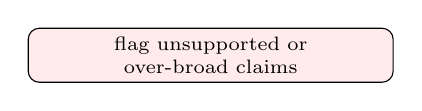
\begin{tikzpicture}
\node[draw,rounded corners,fill=red!8,text width=44mm,align=center,font=\scriptsize] {flag unsupported or over-broad claims};
\end{tikzpicture}
\end{center}
\end{columns}
\end{frame}

\begin{frame}{Tool chains are replaceable components, not the architecture}
\small
\begin{columns}[T,onlytextwidth]
\column{.31\textwidth}
\begin{block}{SDKs}
\scriptsize
Call services directly; choose and connect every component yourself.
\begin{itemize}\itemsep.35em
\item \href{https://developers.openai.com/api/docs/libraries}{\textcolor{brand}{\underline{OpenAI SDK}}}
\item \href{https://platform.claude.com/docs/en/cli-sdks-libraries/overview}{\textcolor{brand}{\underline{Anthropic SDK}}}
\item \href{https://ai.google.dev/gemini-api/docs/libraries}{\textcolor{brand}{\underline{Google GenAI SDK}}}
\end{itemize}
\end{block}
\column{.31\textwidth}
\begin{block}{Frameworks}
\scriptsize
Compose integrations and chains; inspect defaults and generated requests.
\begin{itemize}\itemsep.35em
\item \href{https://www.langchain.com/}{\textcolor{brand}{\underline{LangChain}}}
\item \href{https://www.llamaindex.ai/}{\textcolor{brand}{\underline{LlamaIndex}}}
\item \href{https://haystack.deepset.ai/}{\textcolor{brand}{\underline{Haystack}}}
\end{itemize}
\end{block}
\column{.31\textwidth}
\begin{block}{Products}
\scriptsize
Package workflows; still verify sources, permissions, and citations.
\begin{itemize}\itemsep.35em
\item \href{https://notebook.google/}{\textcolor{brand}{\underline{Gemini Notebook}}}
\item \href{https://docs.useanything.com/}{\textcolor{brand}{\underline{AnythingLLM}}}
\item \href{https://aws.amazon.com/bedrock/knowledge-bases/}{\textcolor{brand}{\underline{Bedrock Knowledge Bases}}}
\end{itemize}
\end{block}
\end{columns}
\vspace{.75em}
\centering\small
Every option should make RAG stages, citations, and cross-cutting controls inspectable.\par
\end{frame}

\begin{frame}{A RAG evaluation starts before the demo}
\small
\begin{columns}[T]
\column{.49\textwidth}
\footnotesize
\begin{itemize}\itemsep.2em
\item Stratify the authorized corpus, then generate diverse questions.
\item Score recall, relevance, groundedness, completeness, and safety.
\item Calibrate automated scores with human labels; retain uncertainty.
\item Stress test ambiguous, adversarial, and out-of-distribution inputs.
\item Slice failures by topic, query type, and risk; revise and repeat.
\end{itemize}
\vspace{.3em}
{\tiny\textit{Lecture 7 covers AI evaluation in depth.}}
\column{.47\textwidth}
\centering
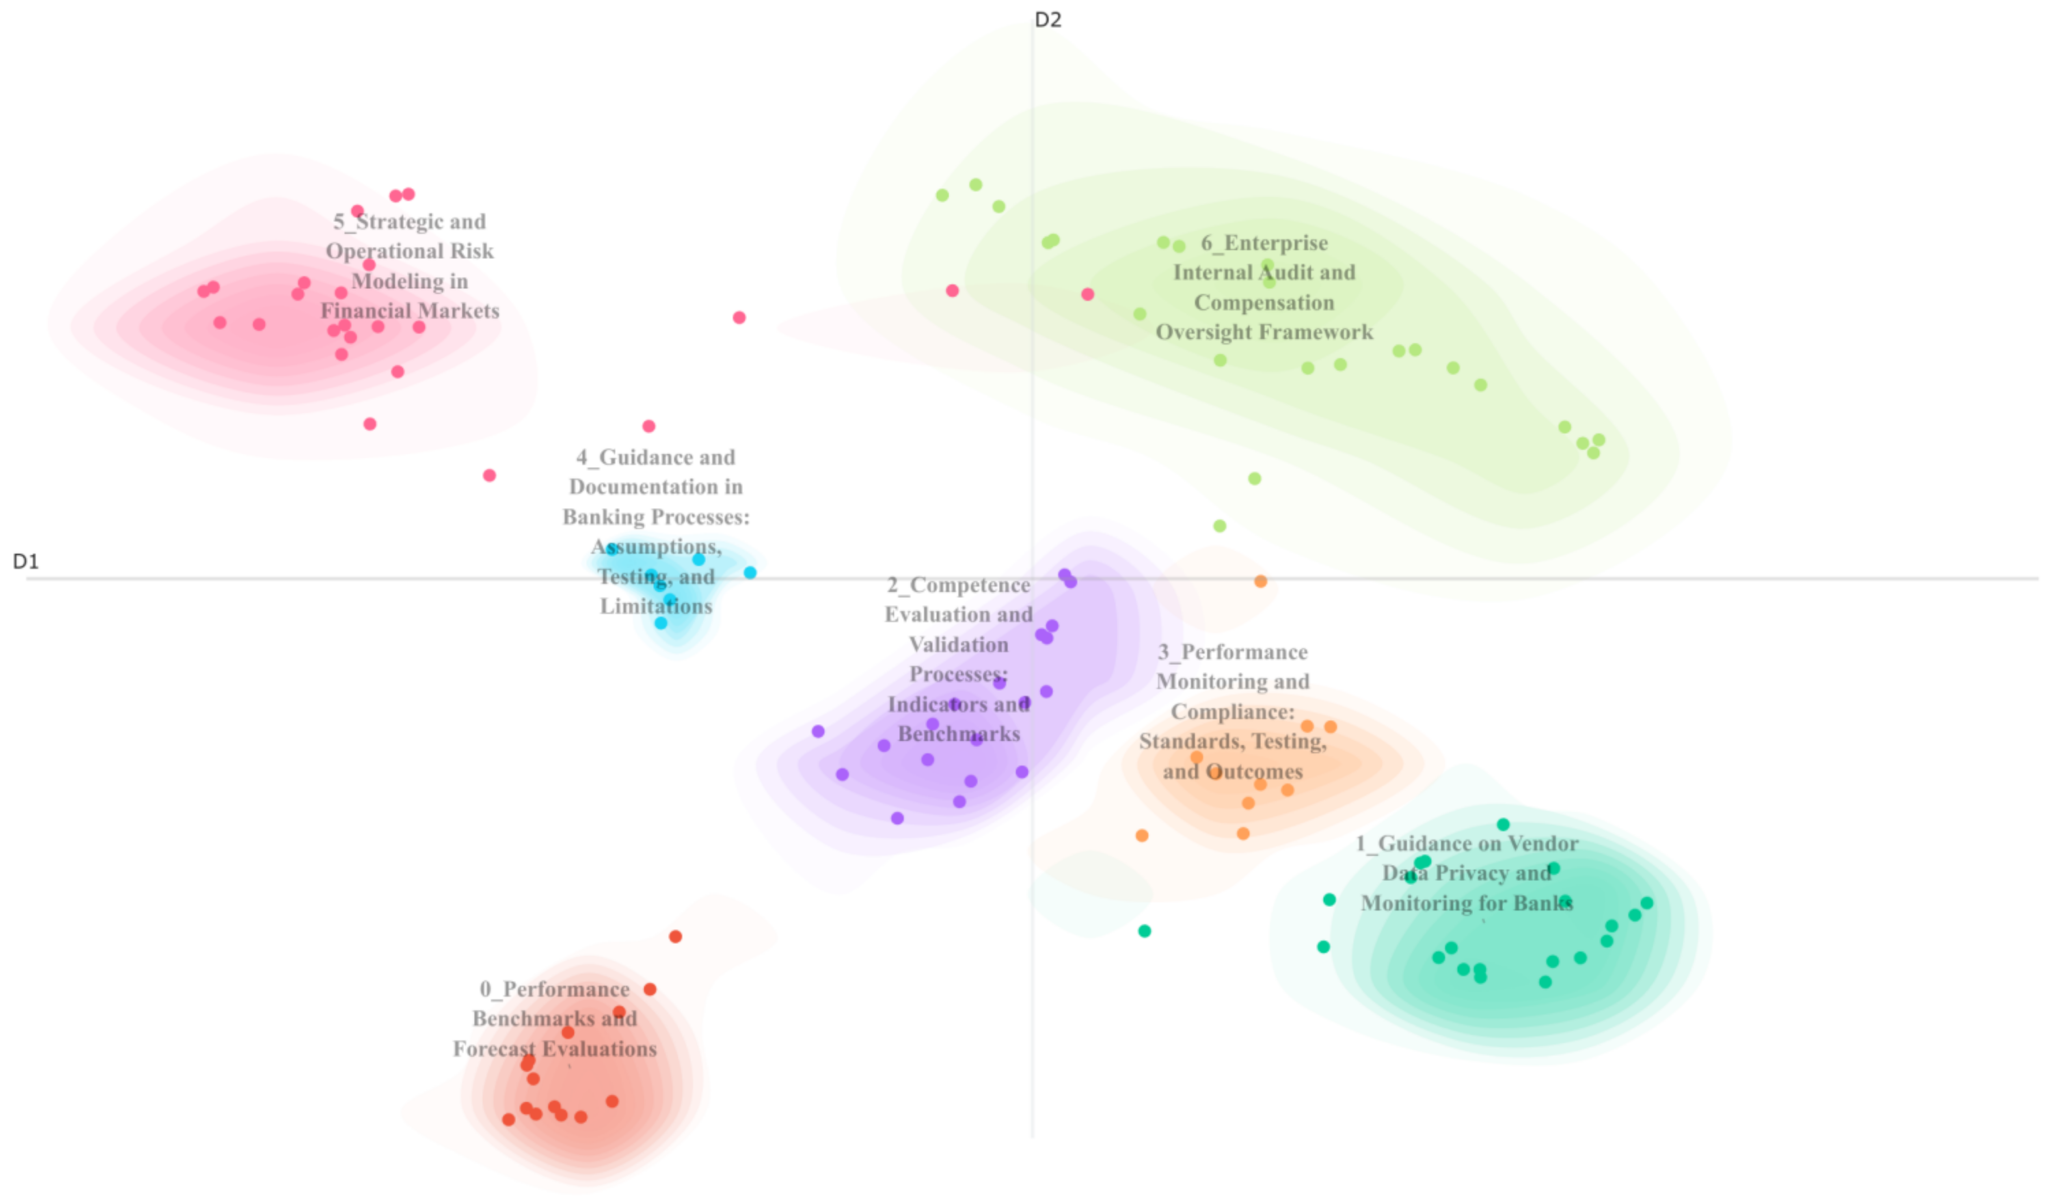
\includegraphics[width=\linewidth,height=.58\textheight,keepaspectratio]{asset/rag.jpg}\\[-.1em]
\scriptsize Source: Sudjianto et al. (2024), \href{https://arxiv.org/abs/2411.16391}{\textit{Human-Calibrated Automated Testing and Validation of Generative Language Models}}.
\par\vspace{.45em}
\visualdescription{Colored clusters illustrate topical strata in a document collection, supporting diverse automated test generation for a RAG system.}
\end{columns}
\end{frame}

\section{Synthesis}
\begin{frame}{Putting the pieces together}
\small
\begin{columns}[c]
\column{.54\textwidth}
\begin{itemize}\itemsep.55em
\item A user makes a query.
\item The retrieval system searches for document chunks similar to the query.
\item The LLM prompt is augmented with the retrieved documents; system instructions provide citation guidelines.
\item The prompt is submitted to the LLM or generation system.
\item A grounded response is generated with citations.
\end{itemize}
\column{.42\textwidth}
\centering
\includegraphics[height=.76\textheight,keepaspectratio]{../../misc/existing_materials/06_GAI Learning - RAG.jpg}\\[.2em]
\parbox{.94\linewidth}{\tiny\raggedright A query retrieves relevant documents, which augment the LLM prompt before a cited answer is generated.}
\end{columns}
\end{frame}

\section{References}
\begin{frame}[t]{References}
\printbibliography[heading=none,keyword=academic]
\end{frame}
\begin{frame}[t]{References}
\printbibliography[heading=none,keyword=documentation]
\end{frame}
\end{document}
